\section{汽化}\label{sec:4-3}

物质从液态变成气态的现象叫做\textbf{汽化}。汽化有两种方式:蒸发和沸腾。

\xiaobiaoti{蒸发}
我们知道,洗过的湿衣服,能晒干也能晾干。
放在敞口容器里的水,过些天会变少。
往碟子里倒一点酒精,很快就干了,并且满屋子都能闻到酒精的气味。
这几个例子里液体都变成了气体,汽化了。
这些汽化现象都是从液体的表面发生的。
只从液体表面发生的汽化现象叫做\textbf{蒸发}。

同样湿的衣服,夏天干得快,冬天干得慢。
这表明液体的温度越高,蒸发得越快。

同样多的水,倒在碟子里干得快,装在瓶子里干得慢。
这表明液体的表面积越大,蒸发得越快。

同样湿的衣服挂在有风的地方干得快,挂在没有风的地方干得慢。
这表明液体表面上的空气流动得越快,蒸发得越快。

可见,为了加快液体蒸发,可以提高液体的温度,增大液体的表面积和加快液体表面上的空气流动。

液体蒸发时还产生一种现象,就是液体的温度降低。这可以从下述的实验看出。
拿两支温度计,用棉花把一支温度计的泡包上,并用温度跟室温相同的酒精把棉花浸湿。
这时棉花上的酒精在蒸发,我们看到,带着湿棉花的温度计表示的温度比另一支温度计的低〈图 \ref{fig:4-3})。

\begin{figure}[htbp]
    \centering
    \begin{minipage}{7cm}
    \centering
    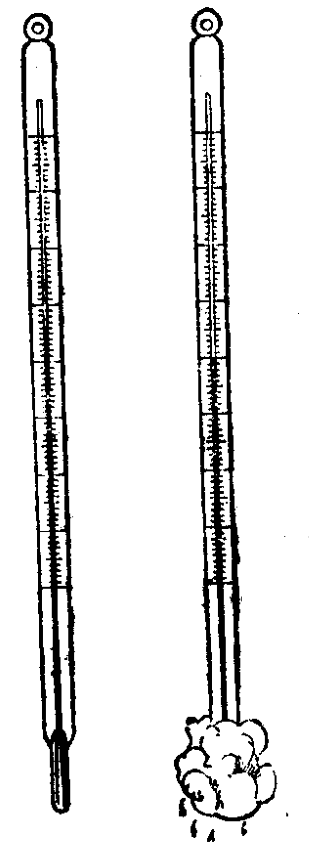
\includegraphics[width=3cm]{../pic/czwl2-ch4-3}
    \caption{液体蒸发时温度降低}\label{fig:4-3}
    \end{minipage}
    \qquad
    \begin{minipage}{7cm}
    \centering
    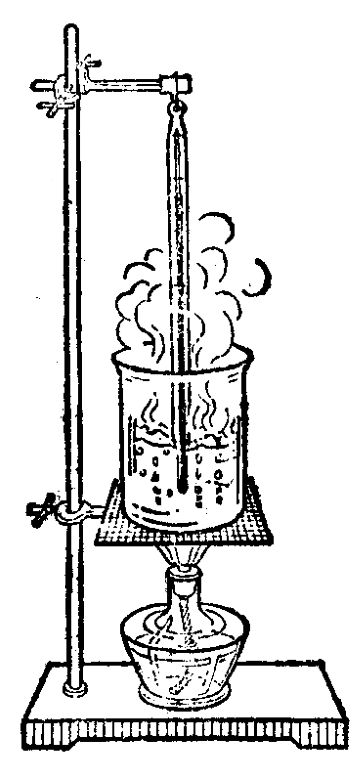
\includegraphics[width=4cm]{../pic/czwl2-ch4-4}
    \caption{水的沸腾}\label{fig:4-4}
    \end{minipage}
\end{figure}

液体蒸发时温度降低,说明它要从周围的物体吸收热量,因此液体蒸发有致冷作用。
在皮肤上擦一点酒精或水,就会感到凉,这是因为酒精或水蒸发时,从身体吸收了热量,使皮肤的温度降低了的缘故。




\xiaobiaoti{沸腾}
把水放在烧杯里加热,当温度升到一定程度时,水中就会发生剧烈的汽化现象,形成大量的汽泡,
上升到水面破裂开来,把里面的水蒸气放掉(图 \ref{fig:4-4}),这种现象叫做\textbf{沸腾}。

蒸发和沸腾这两种汽化现象是有区别的。
蒸发是只在液体表面发生的汽化现象,
沸腾是在液体内部和表面上同时发生的剧烈的汽化现象。

\begin{wrapfigure}{r}{6cm}
    \centering
    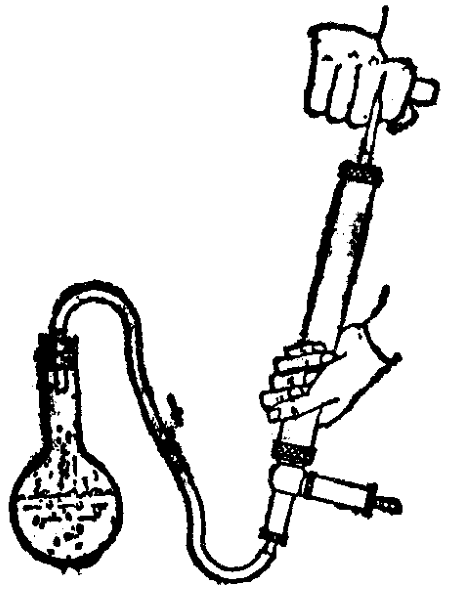
\includegraphics[width=5cm]{../pic/czwl2-ch4-5}
    \caption{水在低压下沸腾}\label{fig:4-5}
\end{wrapfigure}

在图 \ref{fig:4-4} 的实验里,把温度计插入水里来观察水在沸腾时的温度,可以看到水在沸腾过程中,
虽然对它继续加热,它的温度却保持不变。这表明液体是在一定的温度下沸腾的。
沸腾只在一定温度下发生,而蒸发在任何温度下都能发生,这也是它们的区别。

液体沸腾时的温度叫做\textbf{沸点}。不同的液体沸点不同。
即使同一种液体,它的沸点也要随液面上的气压而改变。
在瓶里装入低于 100 ℃ 的水,抽出瓶里的空气,使气压降低,
就会看到水也会沸腾起来(图 \ref{fig:4-5})。
这表明,在压强减小的时候,液体的沸点降低。
相反,如果增加压强,液体的沸点就要升高。

可见,液体的沸点跟压强有关系。
压强增大,沸点升高;
压强减小,沸点降低。

液体的沸点随压强而改变的现象有许多实际应用。
在火力发电厂的锅炉里,要在高压下给水加热,使水的沸点升高,以便得到高温高压的水蒸气。
日常生活里用的高压锅,也是利用高压下沸点升高的道理来更快地煮熟饭菜的。


\begin{table}[H]
    \centering
    \caption*{几种液体在1 标准大气压下的沸点(℃)}
    \begin{tblr}{
        colspec={|ll|ll|ll|},
        columns={colsep+=0.5em},
        column{2,4,6}={mode=math},
    }
        \hline
        液态铁 & 2750 & 水 & 100 & 液态氧 & -183 \\
        液态铅 & 1740 & 酒精 & 78 & 液态氮 & -196 \\
        水银 & 357 & 乙醚 & 35 & 液态氢 & -253 \\
        萘 & 218 & 液态氨 & -33 & 液态氦 & -268.9 \\
        \hline
    \end{tblr}
\end{table}


\xiaobiaoti{汽化热}
液体蒸发时要吸收热量。液体在沸腾过程中,虽然对它继续加热,
但是它的温度保持不变,这就是说液体沸腾时也要吸收热量。
单位质量的某种液体变成同温度的气体时吸收的热量,叫做这种液体的\textbf{汽化热}。
例如,水的汽化热在 100 ℃ 时是 539 卡/克,
即 1 克 100 ℃ 的水变成 100 ℃ 的水蒸气吸收 539 卡的热量。



\lianxi

(1) 晒粮食时,为什么要把粮食放在向阳的地方,并把粮食摊开?

(2) 在刮风时,土地容易变干,但塑料大棚里的土地不容易变干。为什么?

(3) 夏天扇扇子,空气的温度并没有降低,为什么会感到凉爽些?

(4) 有一种粘木料用的胶,需要在 100 ℃ 左右的温度下熬化后才能使用,温度再高就会熬焦,失去粘性。
所以熬这种胶最好用图 \ref{fig:4-6} 所示的两层锅,两层锅之间装着水,这样就不会把胶熬焦了,为什么?

(5) 在高山上用普通的锅煮鸡蛋,水烧开很久,鸡蛋也煮不熟,为什么?怎样才能把鸡蛋煮熟?

(6) 在制糖工业中,要用沸腾的办法除去糖汁中的水分。
为了使糖在沸腾的时候不致变质,沸腾的温度要低于100 ℃ 。想想看,怎样可以做到这一点。

(7) 火箭在大气中飞行时,它的头部跟空气摩擦而产生大量的热,会因温度过高而烧坏。
在火箭头部涂上一层特殊材料,这种材料在高温下熔解并汽化,就能起到保护火箭头部的作用,为什么?


\begin{figure}[htbp]
    \centering
    \begin{minipage}{7cm}
    \centering
    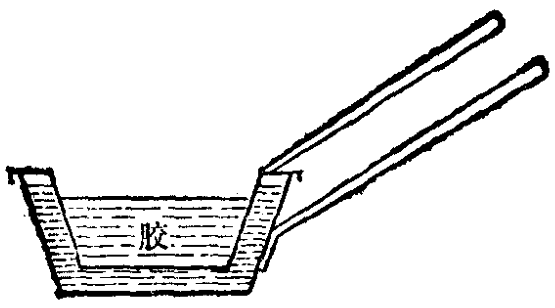
\includegraphics[width=6cm]{../pic/czwl2-ch4-6}
    \caption{熬胶锅}\label{fig:4-6}
    \end{minipage}
    \qquad
    \begin{minipage}{7cm}
    \centering
    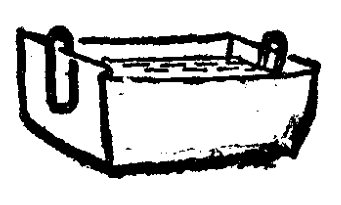
\includegraphics[width=5cm]{../pic/czwl2-ch4-7}
    \caption{烧开水用的纸盒}\label{fig:4-7}
    \end{minipage}
\end{figure}


\section*{小实验}

你相信能用纸盒把水烧开吗?

用一张表面光滑的厚纸做成一个小纸盒,用曲别针把它夹住(图 \ref{fig:4-7})。
纸盒里装些水,放到火上加热。
注意不要让火苗烧到水面以上的纸盒,过一会水就会沸腾起来,而纸盒不会烧着。

你实际做一做,并说明为什么纸盒不会烧着。

